\chapter{Problem Description}
Consider a thin film of Silicon with height $H$ and length $L$. All the loadings and geometry are independent of the third direction; hence, the problem is formulated using the plane strain assumption. There is an existing solid electrolyte interphase (SEI) layer on top of the Silicon film with a height of $H_{\rm{SEI}}$. The origin is placed at the middle of the bottom face of the Silicon film, as shown in figure \ref{fig:probDesc}. The Si thin film's bottom face is considered rigidly fixed to a metallic substrate. The left and right faces are considered to have a roller-type boundary condition for both Si and SEI. A uniform flux of Li-ions from the top surface of SEI is present. 
\begin{figure}[H]
    \centering
    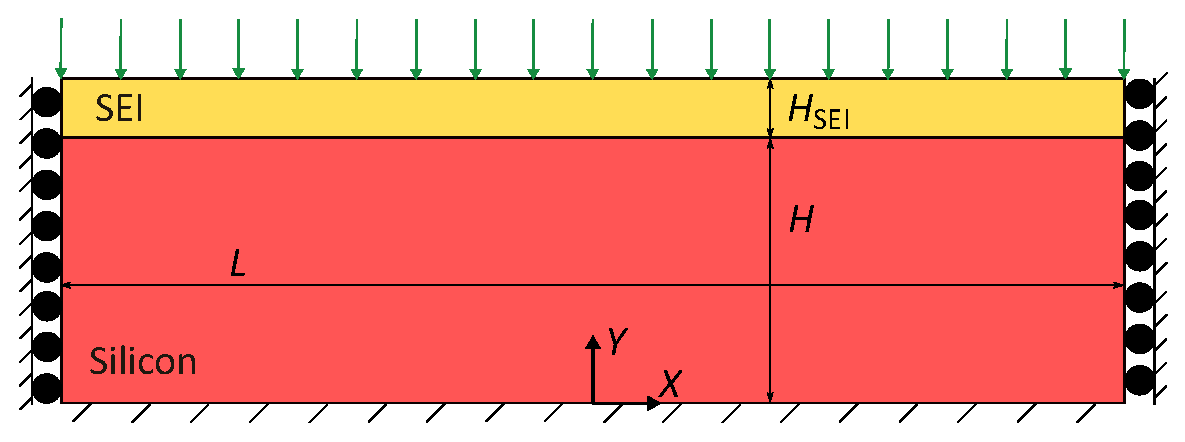
\includegraphics[width=\textwidth]{figures/probDescFigs/drawing.eps}
    \caption{Schematic of the problem showing geometric parameters and boundary conditions.}
    \label{fig:probDesc}
\end{figure}
SEI is considered completely permeable to Li-ions and thus does not undergo deformation due to lithiation. In the Silicon thin film, the diffusion leads to a stress field. In the literature, this is termed diffusion-induced stress (DIS). The stress field, in turn, affects the process of diffusion called stress-enhanced diffusion (SED). This leads to a two-way coupled system of PDEs.
Due to the large deformation of the Si during lithiation, it is necessary to formulate the problem with finite deformation theory with an elastoplastic constitutive behavior. In the present study, both Si and SEI are considered to exhibit a viscoplastic nature. The constitutive law for the elastic regime is isotropic and concentration-dependent for Silicon film and constant for SEI. 
For Mechanical equilibrium, a quasi-static model is employed.